\documentclass[10pt]{article}
\usepackage[spanish,activeacute]{babel}
\usepackage{graphicx}
\usepackage[margin=3cm]{geometry}
\title{\bfseries\Huge Puzlive 1.0\\ Experiencias del Proyecto}
\author{Leonardo Tamayo \\Pedro Iñiguez \\Carlos Caicedo}
\date{}
\begin{document}
\begin{minipage}{0.65\textwidth}
\begingroup
\let\center\flushleft
\let\endcenter\endflushleft
\maketitle

\endgroup
\end{minipage}
\begin{minipage}{0.3\textwidth}

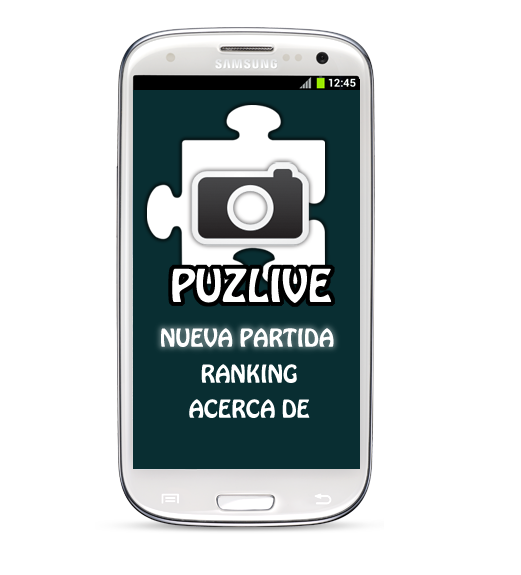
\includegraphics[height=7cm,width=6cm]{androidpro4.png}
\end{minipage}

\section{Leonardo Tamayo}


	
\section{Pedro Iñiguez}
Realmente, armar el proyecto fue una tarea muy dificil. Sin duda alguna representaba un reto muy grande el adaptarse a un nuevo entorno, una nueva libreria, un nuevo IDE, para
poder porgramar en Android. Una experiencia realmente dura buscar como obtener los parametros que devuelven los widgets de los smarthphones, manipularlos, mostrar cosas.
Sin duda muchos tutoriales sirvieron, muchas paginas nos ayudaron y, aunque Leonardo destaco con el arreglo de matrices, cada uno puso su granito de arena en ayudar al otro 
a llenar una parte de la programaci\'on y la documentaci\'on. \\Despues de todo, lo que uno ha aprendido ahora es, ademas de entender el entorno de android, es a poder adaptarse
a algo nuevo y buscar soluciones para optimizar un aprendizaje un desarrollo exitoso.
	

\section{Carlos Caicedo}
	
		


\end{document}